% Copyright (c)  2005-2010 EDF-EADS-PHIMECA.
% Permission is granted to copy, distribute and/or modify this document
% under the terms of the GNU Free Documentation License, Version 1.2
% or any later version published by the Free Software Foundation;
% with no Invariant Sections, no Front-Cover Texts, and no Back-Cover
% Texts.  A copy of the license is included in the section entitled "GNU
% Free Documentation License".
\renewcommand{\filename}{docUC_InputWithData_NormalFittingTests.tex}
\renewcommand{\filetitle}{UC : Normal distribution fitting test, visual validation tests (Henry line) and numerical validation tests in extreme zones (Anderson Darling test and Cramer Von Mises test)}

% \HeaderNNIILevel
% \HeaderIILevel
\HeaderIIILevel


\index{Fitting Test!Henry line}
\index{Fitting Test!Anderson Darling}
\index{Fitting Test!Cramer Von Mises}
\index{Graph!Henry line}
\index{Graph!QQ-plot}
\index{Graph Manipulation!Bounding box}
\index{Graph Manipulation!ViewImage}
\index{Graph Manipulation!Show}

The objective of this Use Case is to fit a normal distribution to a scalar numerical sample, with the maximum likelihood principle or the moment based method, and to validate it with visual and numerical tests.\\

Details on the Maximum Likelihood  Principle may be found in the Reference Guide (\href{OpenTURNS_ReferenceGuide.pdf}{see files Reference Guide - Step B -- Maximum Likelihood  Principle}).\\

Details on the Anderson Darling, Cramer Von Mises and Henry line tests  may be found in the Reference Guide (\href{OpenTURNS_ReferenceGuide.pdf}{see file Reference Guide - Step B -- Anderson Darling goodness-of-fit test, Step B -- Cramer Von Mises goodness-of-fit test and Step B -- Graphical goodness-of-fit tests : QQ-plot and Henry line}).\\

Details on each object may be found in the User Manual  (\href{OpenTURNS_UserManual_TUI.pdf}{see User Manual - Statistics on sample / Distribution factory and / Fitting test}).\\


To help this decision,  Open TURNS proposes the following tests :
\begin{itemize}
\item the Henry line visual test, which is the QQ-Plot graph adapted to the normal distribution,
\item the Anderson Darling test : this test gives more importance to extreme values. If $F_n$ is the empirical cumulative density function of the sample $(x_i)_{1 \leq i \leq n}$ and if $(x_{(i)})_{1 \leq i \leq n}$ is the ordered sample, the Anderson Darling test evaluates the decision variable :
  $$
  \begin{array}{lcl}
    AD^2 & = & \displaystyle  n \int_{\mathbb{R}} \frac{(F_n(x) - F(x))^2}{f(x)(1-F(x))} dF(x)\\
    & = &  \displaystyle -n -\frac{1}{n} \sum_{i=1}^{i=n} (2i-1)[\log(f(x_{(i)})) + \log(1-F(x_{(n-i+1)}))]
  \end{array}
  $$
  Under the hypothesis of normality of the distribution $F$, the decision variable has a tabulated distribution.
\item the Cramer Von Mises test : this test gives also more importance to extreme values. If $F_n$ is the empirical cumulative density function of the sample $(x_i)_{1 \leq i \leq n}$ and if $(x_{(i)})_{1 \leq i \leq n}$ is the ordered sample, the Cramer Von Mises test evaluates the decision variable :
  $$
  \begin{array}{lcl}
    CM & = & \displaystyle  \int_{\mathbb{R}}(F_n(x) - F(x))^2dF(x)\\
    & = &  \displaystyle \frac{1}{12n} + \sum_{i=1}^{i=n} \left[\frac{2i-1}{2n} - F(x_{(i)}) \right]^2
  \end{array}
  $$
  Under the hypothesis of normality of the distribution $F$, the decision variable has a tabulated distribution.
\end{itemize}

\requirements{
  \begin{description}
  \item[$\bullet$] a scalar numerical sample (data)  : {\itshape sample}
  \item[type:]  NumericalSample
  \end{description}
}
{
  \begin{description}
  \item[$\bullet$] a normal fitted distribution : {\itshape estimatedNormalDistribution}
  \item[type:]  Distribution
  \item[$\bullet$] the files containing the Henry line graph : {\itshape HenryPlot.png, HenryPlot.eps}
  \item[type:] files at format PNG or EPS or FIG
  \item[$\bullet$] a numerical validation by the Anderson Darling test for two continuous distributions (p-value)
  \item[type:] TestResult
  \item[$\bullet$] a numerical validation by the  test for Cramer Von Mises discrete distribution (p-value)
  \item[type:] TestResult
  \end{description}
}

\textspace\\
Python script for this UseCase :

\begin{lstlisting}
  # Henry line graph
  # Generate the Graph structure for the Henry line graph
  henryPlot = VisualTest.DrawHenryLine(sample)

  # Impose a bounding box : x-range and y-range
  # boundingBox = [xmin, xmax, ymin, ymax]
  myBoundingBox = NumericalPoint( (xmin, xmax, ymin, ymax) )
  henryPlot.setBoundingBox(myBoundingBox)

  # In order to see the graph without creating the associated files
  Show(henryPlot)

  # Draw the graph on the file HenryPlot.png and HenryPlot.eps
  # if the file adress is not fulfilled, the file is created in the current directory
  henryPlot.draw("HenryPlot")

  # View the bitmap file
  ViewImage(HenryPlot.getBitmap())

  # Check if it worked
  print "bitmap = ", HenryPlot.getBitmap()
  print "postscript = ", HenryPlot.getPostscript()

  # Anderson Darling Test
  # Test = True <=> the sample follows a Normal distribution (H0 hypothesis)
  # p-value threshold : probability of the H0 reject zone = 1-0.95
  # p-value : probability (test variable decision > test variable decision evaluated on the samples)
  # Test = True (=1) <=> p-value > p-value threshold
  # Number of parameters estimated from sample : 4
  resultAndersonDarling =  NormalityTest.AndersonDarlingNormal(sample, 0.95)

  # Print result of the  Anderson Darling Test
  print "Test Succes ? ", (resultAndersonDarling.getBinaryQualityMeasure()==1)

  # Get the p-value of the Anderson Darling Test
  print "p-value of the Anderson Darling Test = ", resultAndersonDarling.getPValue()

  # Get the p-value threshold of the Anderson Darling Test
  print "p-value threshold = ", resultAndersonDarling.getThreshold()

  # Cramer Von Mises Test
  # Test = True <=> the sample follows a Normal distribution (H0 hypothesis)
  # p-value threshold : probability of the H0 reject zone = 1-0.95
  # p-value : probability (test variable decision > test variable decision evaluated on the samples)
  # Test = True (=1) <=> p-value > p-value threshold
  # Number of parameters estimated from sample : 4
  resultCramerVonMises =  NormalityTest.CramerVonMisesNormal(sample, 0.95)

  # Print result of the Cramer Von Mises Test
  print "Test Succes ? ", (resultCramerVonMises.getBinaryQualityMeasure()==1)

  # Get the p-value of the Cramer Von Mises Test
  print "p-value of the Cramer Von Mises Test = ", resultCramerVonMises.getPValue()

  # Get the p-value threshold of the Cramer Von Mises Test
  print "p-value threshold = ", resultCramerVonMises.getThreshold()
\end{lstlisting}

\textspace\\
Figures \ref{henryLineExRight} and \ref{henryLineExFalse} show the Henry Line of a sample coming from a  :
\begin{itemize}
\item  Normal($\mu$ = 0.0, $\sigma$ = 1.0) distribution : visual validation of the normality,
\item  Beta(r = 0.7, t = 1.6, a = 0.0, b = 2.0) distribution : visual invalidation of the normality.
\end{itemize}



\begin{figure}[H]
  \begin{minipage}{10cm}
    \begin{center}
      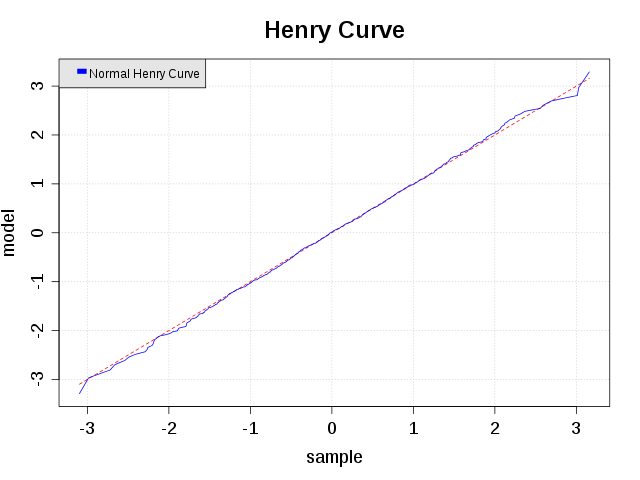
\includegraphics[width=7cm]{HenryLineTestRight.png}
      \caption{Validation of the hypothesis of normality by the Henry Line for a Normal-sample.}
      \label{henryLineExRight}
    \end{center}
  \end{minipage}
  \hfill
  \begin{minipage}{10cm}
    \begin{center}
      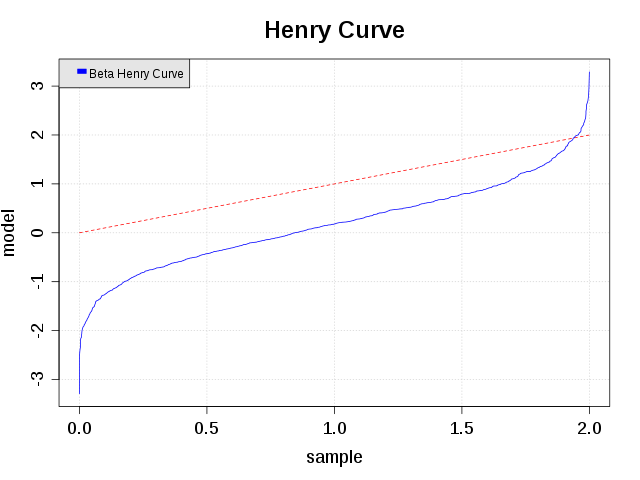
\includegraphics[width=7cm]{HenryLineTestFalse.png}
      \caption{Invalidation of the hypothesis of normalityHenry Line for a Beta-sample.}
      \label{henryLineExFalse}
    \end{center}
  \end{minipage}
\end{figure}

